\documentclass{report}
\usepackage{graphicx}
\graphicspath{{./images/}}
\usepackage[nottoc]{tocbibind}
\usepackage{blindtext}
\usepackage{booktabs}% http://ctan.org/pkg/booktabs
\newcommand{\tabitem}{~~\llap{\textbullet}~~}
\usepackage{geometry}
\geometry{
	a4paper,
	total={170mm,257mm},
	left=30mm,
	right=30mm,
	top=20mm,
}
\usepackage{array}

\begin{document}
	\begin{titlepage}
		\centering
		
\includegraphics[width=0.5\textwidth]{unipi.png}\par\vspace{1cm}
		{\scshape\LARGE Department of Information Engineering \par}
		\vspace{1cm}
		{\huge\bfseries Information Systems \par Task 0 Documentation  \par}
		\vspace{2cm}
		\vfill
		{\Large\scshape Students: \par 
			Adriano Botti \par
			Antonio Le Caldare \par
			Francesco Merola \par 
			Giacomo Ponziani \par}
		\vfill
		
	\end{titlepage}
\tableofcontents
\newpage
\listoffigures

\addcontentsline{toc}{chapter}{Application Specifications}
\chapter*{Application Specifications}
The goal of the application that we implemented is to provide a way for both students and professors to manage the registration process for exams. More specifically, we want the application to exert the following functionalities:
\begin{itemize}
	\item For Students:
	\begin{enumerate}
		\item Check past exams results
		\item Register to an exam date
		\item Delete an exam registration
	\end{enumerate}
	\item For Professors:
	\begin{enumerate}
		\item Add grades to an exam
		\item Create a new exam date
	\end{enumerate} 
\end{itemize}
The application is realized using the Java language, with the JavaFX extension to manage a graphic interface. The back-end uses a MySQL database to store the information.

\addcontentsline{toc}{chapter}{Requirements and Use Cases}
\chapter*{Requirements and Use Cases}
\addcontentsline{toc}{section}{Functional Requirements}
\section*{Functional Requirements}
The Professor:
\begin{enumerate}
	\item shall be able to insert an exam, associated with a course he holds, in a date of choice
	\item shall not be able to inster an exam for a date precedent to the current date
	\item shall be able to insert the corresponding grade for a student in his registration for that exam.
	\item shall insert all grades in the exact date of the exam
\end{enumerate}
The Student:
\begin{enumerate}
	\item shall be able to check the results of past exams
	\item shall be able to register to an exam not yet took
	\item shall not be able to register to an exam after the exam date.
	\item shall be able to register to more successive exams for the same course
	\item If the student registered to successive exams for the same course he just got a mark for, then those future registrations shall be deleted
	\item shall be able to deregister from an exam he was previously registered to
	\item shall not be able to deregister from an exam alredy took
	\item shall not be able to deregister from an exam after the exam date.
\end{enumerate}

\section*{Non-Functional Requirements}
For the application we identified Consistency and Availability as the two most important non-functional requirements.
Both the requirements can be satisfied by the use of a RDBMS, since for our application we don't manage high volumes of data. For this reason we employed a MySQL DBMS to implement our back-end
\newpage
\section*{Use Case Diagram}
From the funtional requirements, a Use Case Diagram is derived. For more detail and a step-by-step description of the different scenarios, see chapter \textit{User's Manual}.
\begin{figure}[ht]
	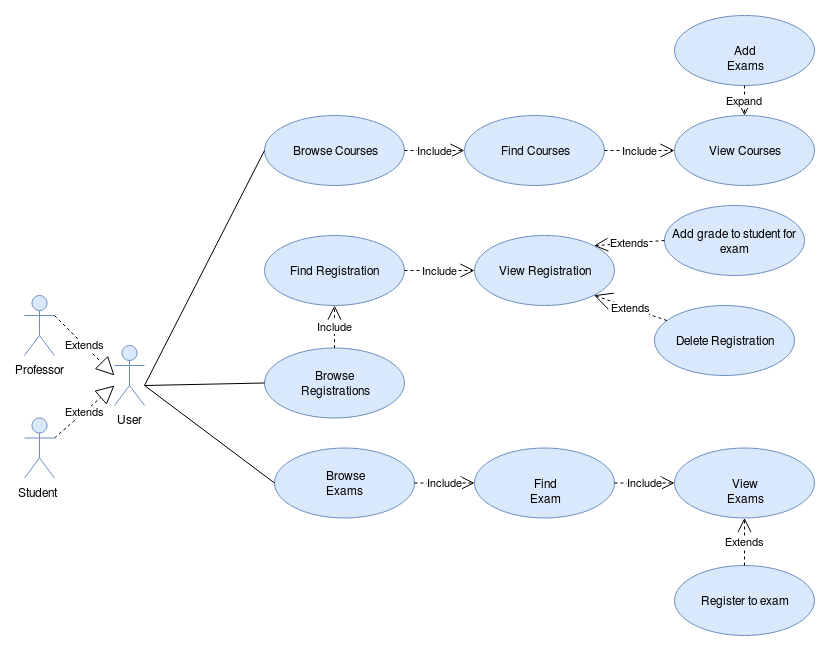
\includegraphics[width=1\textwidth]{UseCaseDiagram.png}
	\caption{Use Cases Diagram}
\end{figure}




\addcontentsline{toc}{chapter}{Entity-Relationship Diagram}
\chapter*{Entity-Relationship Diagram}
\addcontentsline{toc}{section}{ER Vocabulary}
\section*{ER Vocabulary}
\subsection*{Names definition}
Here we define in detail the terms for the main entites and relationships we will use in the following:
\begin{itemize}
	\item \textit{Student}\\ A student is an entity which is able to perform the operations already defined in the requirements. He's an actor for our application. 	
	\item \textit{Professor}\\ A professor is an entity which is able to perform the operations already defined in the requirements. He's an actor for our application. 	
	\item \textit{Course}\\ A course is held by one and only one professor. The course object only includes information about its name, cfu and the helding professor. It holds no information about when exams for that course will take place. 	
	\item \textit{Exam}\\ An exam represents the actual date of the examination for a course.
	\item \textit{Exam Result} An exam result relates an exam to all the students who registered to that exam, adding the information of the grade, if meaningful.\\
\end{itemize} 

\subsection*{Entities}
\begin{table}[ht]
	\centering
	\begin{tabular}{| m{6em} | m{15em} | m{8em} |}
		\hline
		\textbf{Entity} & \textbf{Description} & \textbf{Attributes} \\
		\hline
		Student & Holds all the information related to the students & 
		\tabitem $\underline{id}$ \\
		 & &\tabitem $name$ \\
		 & &\tabitem $surname$ \\
		\hline
		Professor & Holds all the information related to the professors & 
		\tabitem $\underline{id}$ \\
		& &\tabitem $name$ \\
		& &\tabitem $surname$ \\
		\hline
		Course & Holds the information related to the courses & 
		\tabitem $\underline{id}$ \\
		& &\tabitem $name$ \\
		& &\tabitem $cfu$ \\
		& &\tabitem $professor$ \\
		\hline
		Exam & Holds all the new and past exams& 
		\tabitem $\underline{course (ext)}$ \\
		& &\tabitem $\underline{date}$ \\
		\hline
	\end{tabular}
\end{table}

\newpage

\subsection*{Relationships}
\begin{table}[h]
	\centering
	\begin{tabular}{| m{6em} | m{14em} | m{8em} | m{7em} |}
		\hline
		\textbf{Relationship} & \textbf{Description} & \textbf{Participants} & \textbf{Attributes} \\
		\hline
		Teaching & Links Professors to their held courses & 
		\tabitem Professor(1,N) & \\ & &
		\tabitem Course(1,1) & \\
		\hline
		Exam Result & Links students to exams, with the respective grade & 
		\tabitem Student(0,N) & \tabitem $grade$ \\ & &
		\tabitem Exam(0,N) & \\
		\hline
		Exam Date Creation & Links the courses to the exams through a date & 
		\tabitem Course(0,N) & \\ & & 
		\tabitem Exam(1,1) & \\
		\hline
	\end{tabular}
\end{table}
\vspace{5em}
\addcontentsline{toc}{section}{ER Diagram}
\section*{ER Diagram}
\vspace{2em}
\begin{figure}[ht]
	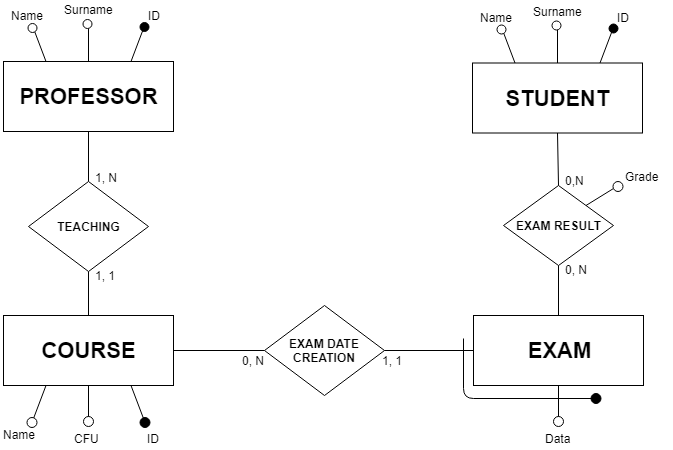
\includegraphics[width=1\textwidth]{ER_Diagram.png}
	\caption{Entity - Relationship Diagram}
\end{figure}

\addcontentsline{toc}{chapter}{UML Class Diagram}
\chapter*{UML Class Diagram} 
\begin{figure}[ht]
	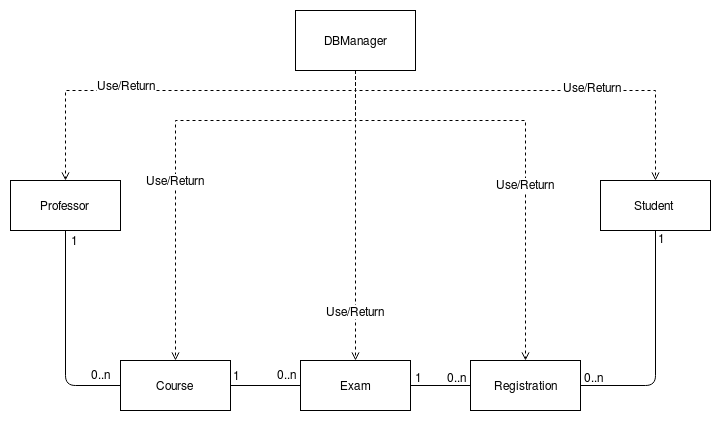
\includegraphics[width=1\textwidth]{ClassDiagram.png}
	\caption{Entity - Relationship Diagram}
\end{figure} 

\addcontentsline{toc}{chapter}{User's Manual}
\chapter*{User's Manual}
The application starts and shows a minimal user interface, fig. \ref{fig:UIStart},
\begin{figure}[h!]
	\centering
	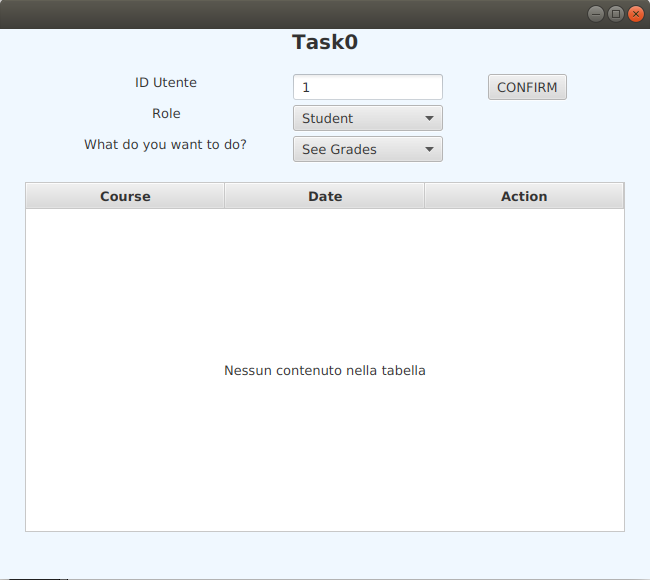
\includegraphics[width=0.7\textwidth]{UIStart.png}
	\caption{User Interface when the application starts}
	\label{fig:UIStart}
\end{figure}
composed of:
\begin{itemize}
	\item \textit{UserID} field, where the user specifies his id number;
	\item \textit{Role} choise box, whith the option:
	\begin{enumerate}
		\item Professor, in case the user is a Professor;
		\item Student, in case the user is a Student.
	\end{enumerate} 
	\item \textit{What do you want to do?} choise box, where the user specifies the action he wants to perform. The options change according to the role chosen.
Professor can select among:
	\begin{enumerate}
		\item \textit{Add Exam} if he wants to add an exam;
		\item \textit{Add Grade} if he wants to add a grade.
	\end{enumerate}
	A Student can select among:
	\begin{enumerate}
		\item \textit{Register to Exam} if he wants to register to an exam;
		\item \textit{Deregister to Exam} if he wants to deregister to an exam;
		\item \textit{See Grades} if he wants to see the grades he got.
	\end{enumerate}
	\item \textit{Confirm} button;
	\item A table showing the results of the selected operation. The layout of the table can change according depending on the selected operation.
\end{itemize}
\section*{Professor}
A Professor:
\begin{enumerate}
	\item Inserts his ID number into the \textit{UserID} field;
	\item Selects \textsl{Professor} in the \textit{Role} choise box;
	\item Selects the action he wants to perform;
	\item Pushes the \textit{Confirm} button.
\end{enumerate}
\subsubsection*{Add Exam}
If the Professor select the \textit{Add Exam} option, the table, fig. \ref{fig:AddExam}, is populated with a list of all the courses he is currently holding. Each element of the list is composed of:
\begin{figure} [h!]
	\centering
	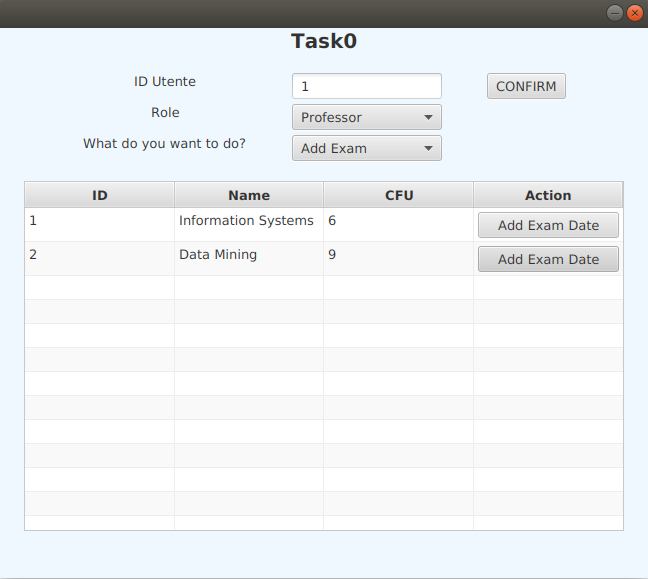
\includegraphics[width=0.7\textwidth]{AddExam.png}
	\caption{Example of Add Exam}
	\label{fig:AddExam}
\end{figure}
\begin{itemize}
	\item \textit{ID}, the id of the course;
	\item \textit{Name}, the name of the course;
	\item \textit{CFU}, the number of credits assigned to the course;
	\item \textit{Add Exam Date}, button the professor has to push in order to add an exam corresponding to the course. 
\end{itemize}

If the Professor pushes one of the \textit{Add Exam Date} buttons a confirm dialog is presented and it asks for the date of the exam to insert, fig. \ref{fig:AddExamDialog}.
\begin{figure} [h!]
	\centering
	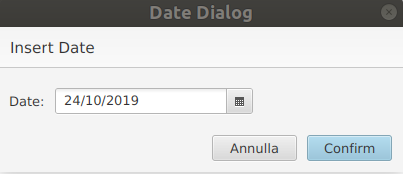
\includegraphics[width=0.5\textwidth]{AddExamDialog.png}
	\caption{Example of Add Exam dialog}
	\label{fig:AddExamDialog}
\end{figure} 
If the Professor wants to confirm he:
\begin{enumerate}
	\item Selects the date using the datepicker;
	\item Pushes the \textit{Confirm} button in the dialog.
\end{enumerate}
To go back and undo the operation the Professor just pushes the \textit{Delete} button.
\subsubsection*{Add Grade}
If the Professor select the \textit{Add Grade} option, the table, fig. \ref{fig:AddGrade}, is populated with a list of all the registrations to the courses he is currently holding. Each element of the list is composed of:
\begin{figure} [h!]
	\centering
	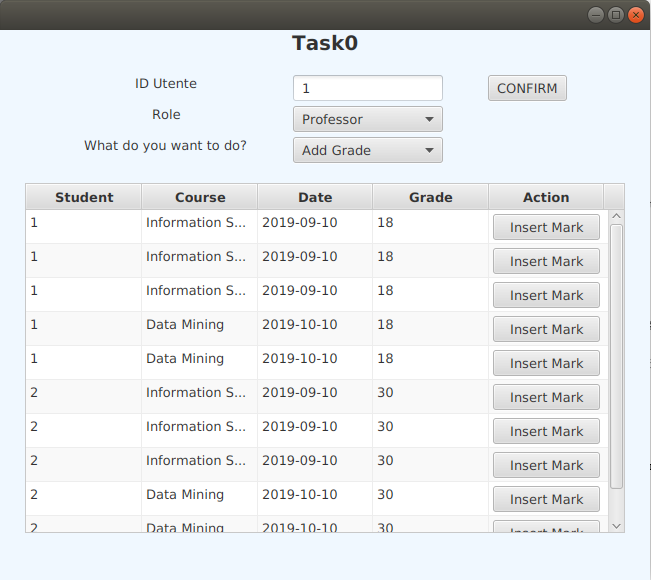
\includegraphics[width=0.7\textwidth]{AddGrade.png}
	\caption{Example of Add Grade}
	\label{fig:AddGrade}
\end{figure}
\begin{itemize}
	\item \textit{Student}, the id of the student enrolled to the exam;
	\item \textit{Course}, the name of the course;
	\item \textit{Date}, the date of the exam;
	\item \textit{Insert Mark} button that the professor has to push in order to insert a grade to the corresponding registration. 
\end{itemize}
If the Professor pushes one of the \textit{Insert mark} buttons a confirm dialog is presented and it asks for the grade of the exam to insert, fig. \ref{fig:AddGradeDialog}.
\begin{figure} [h!]
	\centering
	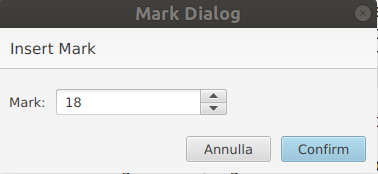
\includegraphics[width=0.5\textwidth]{AddGradeDialog.png}
	\caption{Example of Add Grade dialog}
	\label{fig:AddGradeDialog}
\end{figure}
If the Professor wants to confirm he:
\begin{enumerate}
	\item Inserts the grade in the corresponding field;
	\item Pushes the \textit{Confirm} button in the dialog.
\end{enumerate}
To go back and undo the operation the Professor just pushes the \textit{Delete} button.

\section*{Student}
A Student:
\begin{enumerate}
	\item Inserts his ID number in the \textit{UserID} field;
	\item Selects \textsl{Student} in the \textit{Role} choise box;
	\item Selects the action he wants to perform;
	\item Pushes the \textit{Confirm} button.
\end{enumerate}
\subsubsection*{Register to Exam}
If the Student select the \textit{Register to Exam} option, the table, fig. \ref{fig:RegisterToExam}, is populated with a list of all the available exams. Each element of the list is composed of:
\begin{figure} [h!]
	\centering
	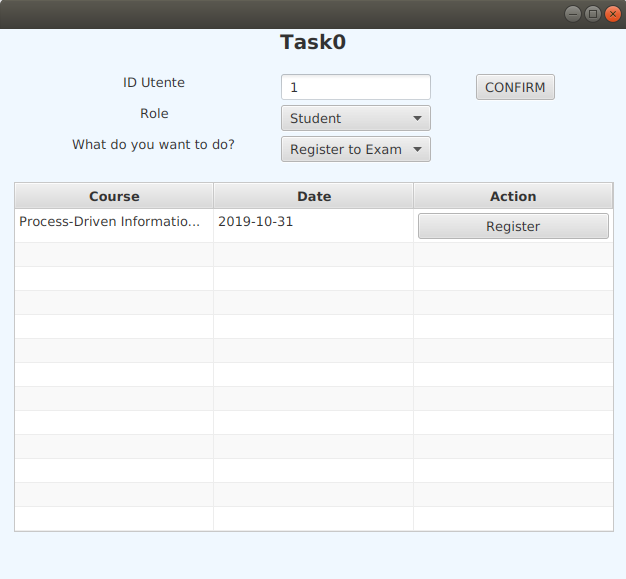
\includegraphics[width=0.7\textwidth]{RegisterToExam.png}
	\caption{Example of Register to Exam}
	\label{fig:RegisterToExam}
\end{figure}
\begin{itemize}
	\item \textit{Course}, the name of the course;
	\item \textit{Date}, the date of the exam;
	\item \textit{Register}, button the student has to push in order to register to the selected exam. 
\end{itemize}
If the Student pushes one of the \textit{Register to Exam} the table is updated so that it shows all the exams to which the Student is not enrolled.

\subsubsection*{Deregister to Exam}
If the Student select the \textit{Deregister} option, the table, fig. \ref{fig:DeregisterToExam}, is populated with a list of all the registrations corresponding to the Student. Each element of the list is composed of:
\begin{figure} [h!]
	\centering
	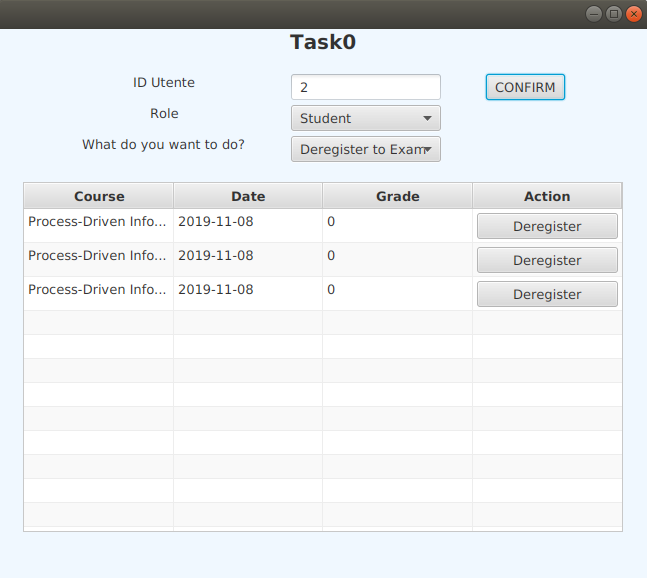
\includegraphics[width=0.7\textwidth]{DeregisterToExam.png}
	\caption{Example of Deregister to Exam}
	\label{fig:DeregisterToExam}
\end{figure}
\begin{itemize}
	\item \textit{Course}, the name of the course of the exam the Student is enrolled to;
	\item \textit{Date}, the date of the exam;
	\item \textit{Deregister} button that the Stuedent has to push in order to do the deregistration. 
\end{itemize}
If the Professor pushes one of the \textit{Deregister} the table is updated so that it shows all the exams to which the Student is not enrolled.

\subsubsection*{See Grades}
If the Student select the \textit{See Grades} option, the table, fig. \ref{fig:SeeGrades}, is populated with a list of all the exams the student has done. Each element of the list is composed of:
\begin{figure} [h!]
	\centering
	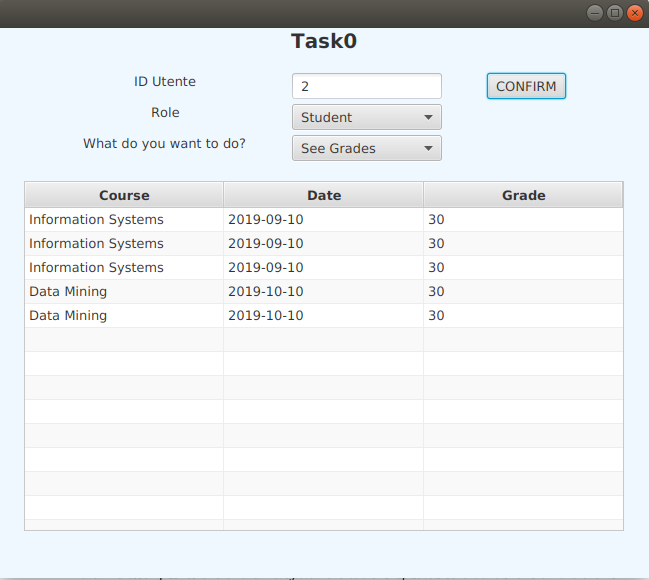
\includegraphics[width=0.7\textwidth]{SeeGrades.png}
	\caption{Example of See Grades}
	\label{fig:SeeGrades}
\end{figure}
\begin{itemize}
	\item \textit{Course}, the name of the course;
	\item \textit{Date}, the date when the student passed the exam;
	\item \textit{Grade}, the grade the Student got. 
\end{itemize}


\begin{thebibliography}{9}
\end{thebibliography}

\end{document}
